\documentclass{standalone}
\usepackage[dvipsnames]{xcolor}
\usepackage{tikz}
\usetikzlibrary{positioning, calc, shapes, fit}

\begin{document}

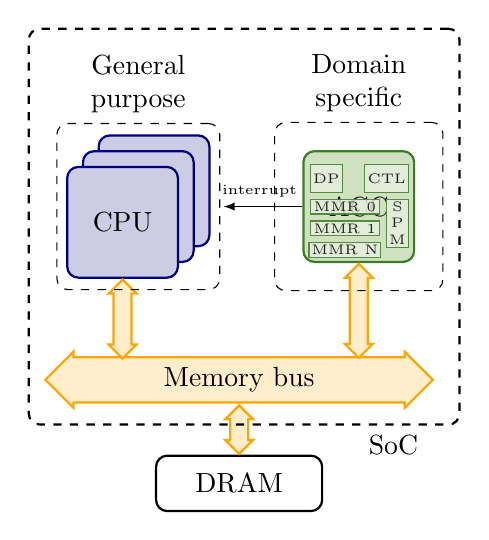
\begin{tikzpicture}
  \tikzstyle{PE}=[rounded corners, draw, thick, minimum size=40pt, align=center]
  \tikzstyle{core}=[PE, draw=NavyBlue, fill=NavyBlue!20]
  \tikzstyle{hwacc}=[PE, draw=OliveGreen, fill=OliveGreen!20]
  \tikzstyle{bus}=[double arrow, draw=Orange, fill=Orange!20, thick,
  minimum width=20pt, double arrow head extend=2pt]
  \tikzstyle{accint}=[draw=OliveGreen, fill=OliveGreen!10, outer sep=1pt, inner sep=1pt,
  node distance=0.5pt, opacity=0.85]

  \begin{scope}[name=soc, local bounding box=socbb]
  \node (core2) at (0.4,0.4) [core] {};
  \node (core1) at (0.2,0.2) [core] {};
  \node (core0) at (0,0) [core] {CPU};

  \node (hwacc1) at (3,0.2) [hwacc] {ACC};
  \begin{scope}[name=completeacc, local bounding box=accbb, shift={(3, 0.2)}]
    \node (reg0) [accint, minimum width=25pt, xshift=-5pt, minimum height=5pt, font=\tiny] {MMR 0};
    \node (reg1) [accint, minimum width=25pt, minimum height=5pt, below=of reg0, font=\tiny] {MMR 1};
    \node (reg2) [accint, minimum width=25pt, minimum height=5pt, below=of reg1, font=\tiny] {MMR N};
    \node (spm) [accint, minimum height=15pt, minimum width=5pt, align=center,
    right=of reg0.north east, font=\tiny, anchor=north west] {S\\P\\M};
    \node (accpe) [accint, minimum width=10pt, minimum height=10pt, above=of reg0.north west,
    anchor=south west, font=\tiny] {DP};
    \node (accctl) [accint, minimum width=10pt, minimum height=10pt, above=of spm.north east,
    anchor=south east, font=\tiny] {CTL};
  \end{scope}
  \node (mainbus) at (-1, -2) [bus, anchor=west, minimum height=140pt] {Memory bus};

  \node at (core0.south) [bus, rotate=90, anchor=east, scale=0.5, minimum height=57pt] {};
  \node at (hwacc1.south) [bus, rotate=90, anchor=east, scale=0.5, minimum height=68pt] {};

  \node (gpc) [fit=(core0)(core1)(core2), rounded corners,
  dashed, draw, minimum height=60pt, label={[align=center]90:{General\\ purpose}}] {};
  \node (dsc) [fit=(hwacc1), rounded corners, dashed, inner sep=10pt,
  draw, minimum height=60pt, label={[align=center]90:{Domain\\ specific}}] {};

  \draw[-latex] (hwacc1.west) -- ++(-1,0) node [anchor=south west, xshift=-4pt] {\tiny interrupt};
  \end{scope}

  \node (dram) [draw, rounded corners, below= of mainbus, minimum width=60pt,
  minimum height=20pt, yshift=10pt, thick] {DRAM};

  \node at (dram.north) [bus, rotate=-90, anchor=east, scale=0.5, minimum height=35pt] {};

  \node [fit=(socbb), draw, dashed, rounded corners, thick, inner sep=6pt, label={300:SoC}] {};

\end{tikzpicture}

\end{document}